\documentclass[10pt]{article}
\usepackage{amsmath}
\usepackage{amsfonts}
\usepackage{amssymb}

\usepackage{graphicx}
\usepackage{caption}
\usepackage{subcaption}
\usepackage{tikz-timing}
\usepackage{tikz}
\usetikzlibrary{shapes,arrows}

\author{Sawaiz Syed}
\title{Networked Radiation Sensors}

\begin{document}
\maketitle

\begin{abstract}
Collecting radiation data is a difficult task as most equipment is costly and custom built. The solution is a Geiger counter that transmits data, and a server that collects it. It provides low per unit cost, and data from many locations.
\end{abstract}

\section{Introduction}
Cosmic ray radiation from outside our solar system are powerful gamma rays that disperse 
after hitting out atmosphere. As we move closer to the edge of our atmosphere, their 
energy increases \cite{Nave}. About 90\% of cosmic rays are protons, and 9\% 
are alpha particles \cite{Nave}. These very high energy particles (called 
primaries)Strike the upper layer of the atmosphere and transfer their energy into 
particles classified as secondaries. The secondary rays consist of pions (that decay 
to muons, neutrinos, and gamma rays) and electrons and positrons \cite{Mewaldt1996}. The 
Figure~\ref{fig:atmosphericCascade} shows the how the atmospheric cascade reduces the energy of 
the primary particle into multiple weaker secondaries, if the energy of the primary 
is above 500MeV, the secondaries will still reach earth's surface before dissipation 
\cite{Bieber2000}. 

\begin{figure}[h]
	\centering
	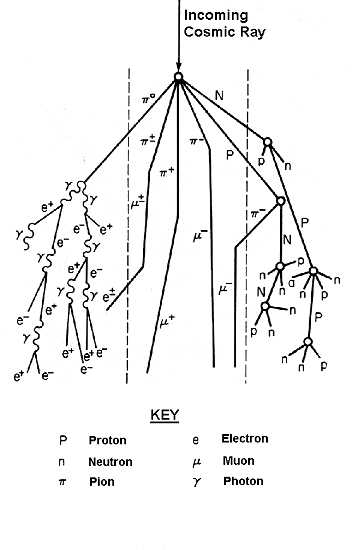
\includegraphics[width=0.5\textwidth]{atmosphericCascade.png}
	\caption{Atmospheric cascade.}
	\label{fig:atmosphericCascade}
\end{figure}

The average energy of primary particles is 1GeV (corresponding to .87C) 
although TeV occurrences have been measured.\cite{Nave}. While at sea level the 
radiation caused by the particles is low with an intensity of $100 \frac{particles}{m^2s}$ 
\cite{Mewaldt1996}, it can still cause memory electronic errors, and health effects to 
aviation \cite{Friedberg2000} and space personnel.

\subsection{Previous Research}
The sensors currently available for radiation detection are expensive, devices made 
once with limited documentation to how they work, and are used. They provide a very 
small set of data, and at only a single location, generally inside a climate controlled 
lab. The devices are designed without the consideration of making more devices, and 
creating additional devices adds greatly to both the cost and time. Previously data 
has been collected and used, but in very limited amounts. The data collected has been 
from distant locations such as the radiation sensor on campus, while the weather 
readings are measured from Peachtree City Observation Station \cite{Dayananda2013}, 
approximately thirty miles away this provides general readings but the weather variance 
can be so great between those locations that precise coloration is difficult to 
accomplish. The newer results use a weather station atop the building, but the sensors 
are physically too close that all the data from the detectors would not give 
information on the larger scale.

\subsection{Infrastructure}
With city infrastructure getting denser and complex, the threat of dirty bombs and 
danger from nuclear power facilities pose a risk in tightly packed urban areas. 
Detecting radiation on such a scale is difficult, expensive, and is difficult to 
justify the cost when the funds can be allocated to other infrastructure. Small 
inexpensive mountable mesh of sensors can provide real time location based
radiation readings and sensors mounted on public transit and government vehicles would also 
provide geolocation data for trackable readings. These could give information critical 
to the current security for anti terrorism, public safety, and long term data that provides information
on how average radiation readings fluctuate.

\subsection{Workplace}
In locations where retroactively hazardous materials could be handled this information can
be helpful to mitigate problems caused by human error. An example scenario could be a worker 
dealing with radioactive materials, leaving the room without placing the sample back into storage.
The system could also warn the personnel overseeing a nuclear power plant of any leaks of contamination
due to the larger amount of area the sensors would cover at the same cost as currently used sensors.

\subsection{Current Options}
The options for the collection of current data has been very sparse. Small hand held sensors can
provide data that would either have to be manually logged, along with the location and hence is 
highly impractical. Other options include addons to weather stations, and computers with many 
sensors connected via USB, and modular sensor systems. But the major problem with 
all these options is the physical size and high power consumption that limits the locations and 
areas the devices can be placed. Most devices have a volume of ten to one hundred times the 
volume of the sensing apparatus, and a power consumption on the order of ten to hundreds of 
milliamps, that is too high for long term data logging.

\subsection{Requirements}
An ideal sensor setup would consist of a physically small sensor with very low power consumption. 
Multiple transmitters with little computing all sending to a single internet connected receiver 
with error checking. It should be physically strong, easily mountable, and weather proof. Finally
the unit should be designed for manufacturing to make the cost per unit as low as possible. The 
device should have good code and hardware documentation for further research and for others to use 
it as a platform for making other sensors.


\section{Methods}
The construction of this sensor will follow a hardware driven methodology
as cost is the major factor in determination of components and functionality.
Everything will be built in a modular fashion to make expansions and future
development simple. The components will be designed in sections talking in power
and signals, or outputting data. 

\subsection{Hardware}
The general build of the hardware will consist of a microcontroller, the acting 
processor, executing code based on inputs and outputs attached. There will be 
sensor attached to multiple pins including temperature, humidity, light, and 
location sensors. The high voltage power supply tuned to hold the a Geiger 
tube at its operating voltage. A sector for collecting and storing power, and 
finally a wireless transmitter. 

\subparagraph{Microcontroller}
The selection of the microcontroller is the factor the rest of the project
will be constructed around. The prototypes were initially made from the ATtiny13A
made by Atmel. It is a eight pin device in package sizes down to $3mm \times3 mm$. 
It was chosen for its low cost, and personal experience with the Atmel's offerings.
As pins ran out and additional functionality was needed, an upgrade to ATtiny24 was
in order, it provided six additional sensor and communication pins. The programming is
done though C and/or Avr assembly, a lower level interface for faster operations.

The receiver is mainly being designed for testing, and will be made in the Arduino 
(a popular prototyping platform based on Atmel microcontrolers) and programmed in C++ 
for quicker prototyping.

\subparagraph{Wireless}
The wireless system will consist of a transmitter on the sensing device communicating at
either 433 MHz or 915 MHz as those are the legal ISM (Industrial, Scientific, Manufacturing) 
frequencies in most of the world. Another option would be the 2.4GHz band, but with a lower 
penetration and a more congested frequency it is a worse option, the lower frequencies have 
enough bandwidth. These bands are FCC compliant to keep certification simple, and the 
transmitter will be using a trace antenna, one that resides only on the circuit board, to 
keep costs low.

\subparagraph{Sensors}
The main requirement of the device is to sense radioactive particles, so a 
Geiger M\"{u}ller tube will be used, the SBM-20 shown in Figure~\ref{sbm20}, a 
Russian tube designed for detecting Hard Beta, and Gama rays. With a manageable 
recommended voltage of 400 V, pulse life of $2 \times 10^{10}$, and ease of 
availability, makes it a great choice \cite{Bodunova-Skvortsova}. Other sensors 
such as a temperature, humidity, and light will be added to provide ambient 
information. GPS sensors will be designed as an expansion module for devices 
that are expected to have changed position after installation, such as those 
on rail.

\begin{figure}[h]
	\centering
	\includegraphics[width=0.5\textwidth]{sbm20}
	\caption{SBM-20 Geiger Muller Tubes \cite{Bodunova-Skvortsova} \label{sbm20}}
\end{figure}

\subparagraph{Power}
Power to the unit will be provided through a lithium ion 3.7V (nominal) battery such 
as those common in consumer electronics. Its safety will be manged by a charging and 
protection chip which will be able to monitor current draw, and provide recharging power 
through a solar panel attached outside the enclosure. The high voltage supply will be a 
simple boost converter (a circuit that uses the voltage rise in inductors to generate 
higher voltages) tuned to the 400V required for the Geiger tube.

\subparagraph{Casing}
Enclosure design will be based around PVC pipe for lower volume and injection molded 
ABS for higher volumes. The pipe is conducive to the long components that take the majority
of the volume of the design. The Tube, and the battery will stack vertically with PCB 
(printed circuit board layers) in the middle very similar to Cordwood construction 
,exampled in Figure~\ref{cordwood}, previously used in missile and telemetry systems 
where space was at a premium. These layers will be connected with long strips of PCB 
material connecting them top provide rigidity and structure and act as power lines. 
The ABS design will be based on ease of mounting and identification of the modules. 

\begin{figure}[h]
	\centering
	\includegraphics[width=0.7\textwidth]{cordwoodcircuit}
	\caption{A circuit built with stacked PCB \cite{ArnoldReinhold} \label{cordwood}}
\end{figure}

\subsection{Software}

Software will be programed in AVR C for the transmitter and C++ and Java for the receiver 
for quicker prototyping. Code flow with be dependent on incoming pulses form the radiation 
detector. Upon receiving the microcontroller will cycle through it's duties shown in 
Figure~\ref{structure} before returning to sleep(the low power mode).

\begin{figure}[h]
	\centering
	
	\tikzstyle{block} = [rectangle, draw, fill=blue!20, 
	text width=5em, text centered, rounded corners, minimum height=4em]
	\tikzstyle{line} = [draw, -latex']
	
	\begin{tikzpicture}[node distance = 3cm, auto]
	
	\node [block] (interupt) {Pin Change Interupt};
	\node [block , right of=interupt] (sensor) {Read Sensors};
	\node [block , right of=sensor] (encode) {Encode data};
	\node [block , below of=encode] (transmit) {Transmit Data};
	\node [block , left of=transmit] (sleep) {Sleep};
	
	\path [line] (interupt)--(sensor);
	\path [line] (sensor)--(encode);
	\path [line] (encode)--(transmit);
	\path [line] (transmit)--(sleep);
	\path [line] (sleep)-|(interupt);
	
	\end{tikzpicture}
	\caption{Software Structure \label{structure}}
\end{figure}

\subparagraph{Encoding}
The receivers auto gain control adjusts to ambient noise level. This means the gain must be
reduced before the first byte can be transmitted. There is a pulse train of square waves 
one unit width in timing that are transmitted before any messages to reduce gain and 
therefore interference. Then a synchronization pulse is sent so the receiver knows where 
to begin timing. The data is sent in a Manchester encoding style as recommended in RF 
Monolithic guide \cite{RFMonolithics}. This forces the output pin to not remain in one state 
for too long causing the gain to not fluctuate as much as it might otherwise by sending 
the inverse of the previous bit for one unit, see Figure~\ref{manchester} as reference. The 
encoded data to send will include ID of the unit (set at  install), the readings from the 
sensors, and calculated parity bits to verify data on the receiving end.

\begin{figure}[h]
	\begin{tikztimingtable}
		Gain Setting						& 20{1C} G\\
		Synchronization Pulse               & L 20H L \\
		Sending 0 (0x00)       		        & LHLHLHLHLHLHLH \\
		Sending L (0x4C)       		        & HLLHLHHLHLLHLH \\
		Sending 255 (0xFF)					& HLHLHLHLHLHLHL \\
	\end{tikztimingtable}
	\caption{Timing Tables of transmitting pulses \label{manchester}}
\end{figure}
\subsection{Testing}
The devices will be range tested at distances of up to 100m for both data integrity, and verification that the majority of pulses that occur are received. With the solar panel, discharge rate and recharging time will be addressed to verify that device will remain 
operable over its lifespan.

\subsection{Production}
Designing for production requires more forethought than when building a one off system.

\subparagraph{Scaling}
The quantity is the major determinate in at what cost you can build your devices. 
Component selection is important as slight cost increases trickle to larger costs. 
The cost assembly and shipping become major expenditures as with smaller runs, the designer
does assembly and shipping is consider to be nominal as it only occurs once. Another 
important aspect during scaling is to consider time required between each step, different 
fabrication facilities have varying fulfillment times.

\subparagraph{Documentation}
Documenting work for future development will be done though a document that explains 
the use and modifications required for it to fit the purpose. The hardware will have 
3D models created for it during development and those will provide diagrams and 
animations for documentation.


\section{Results}
The device, although still under development, has reached a late prototype stage. Many of the design goals set out were reached. Circuits and schematics still need to be finalized therefore testing was completed with the prototypes, Figure~\ref{fig:txrx}. 

\begin{figure}
	\centering
	\begin{subfigure}[b]{0.3\textwidth}
		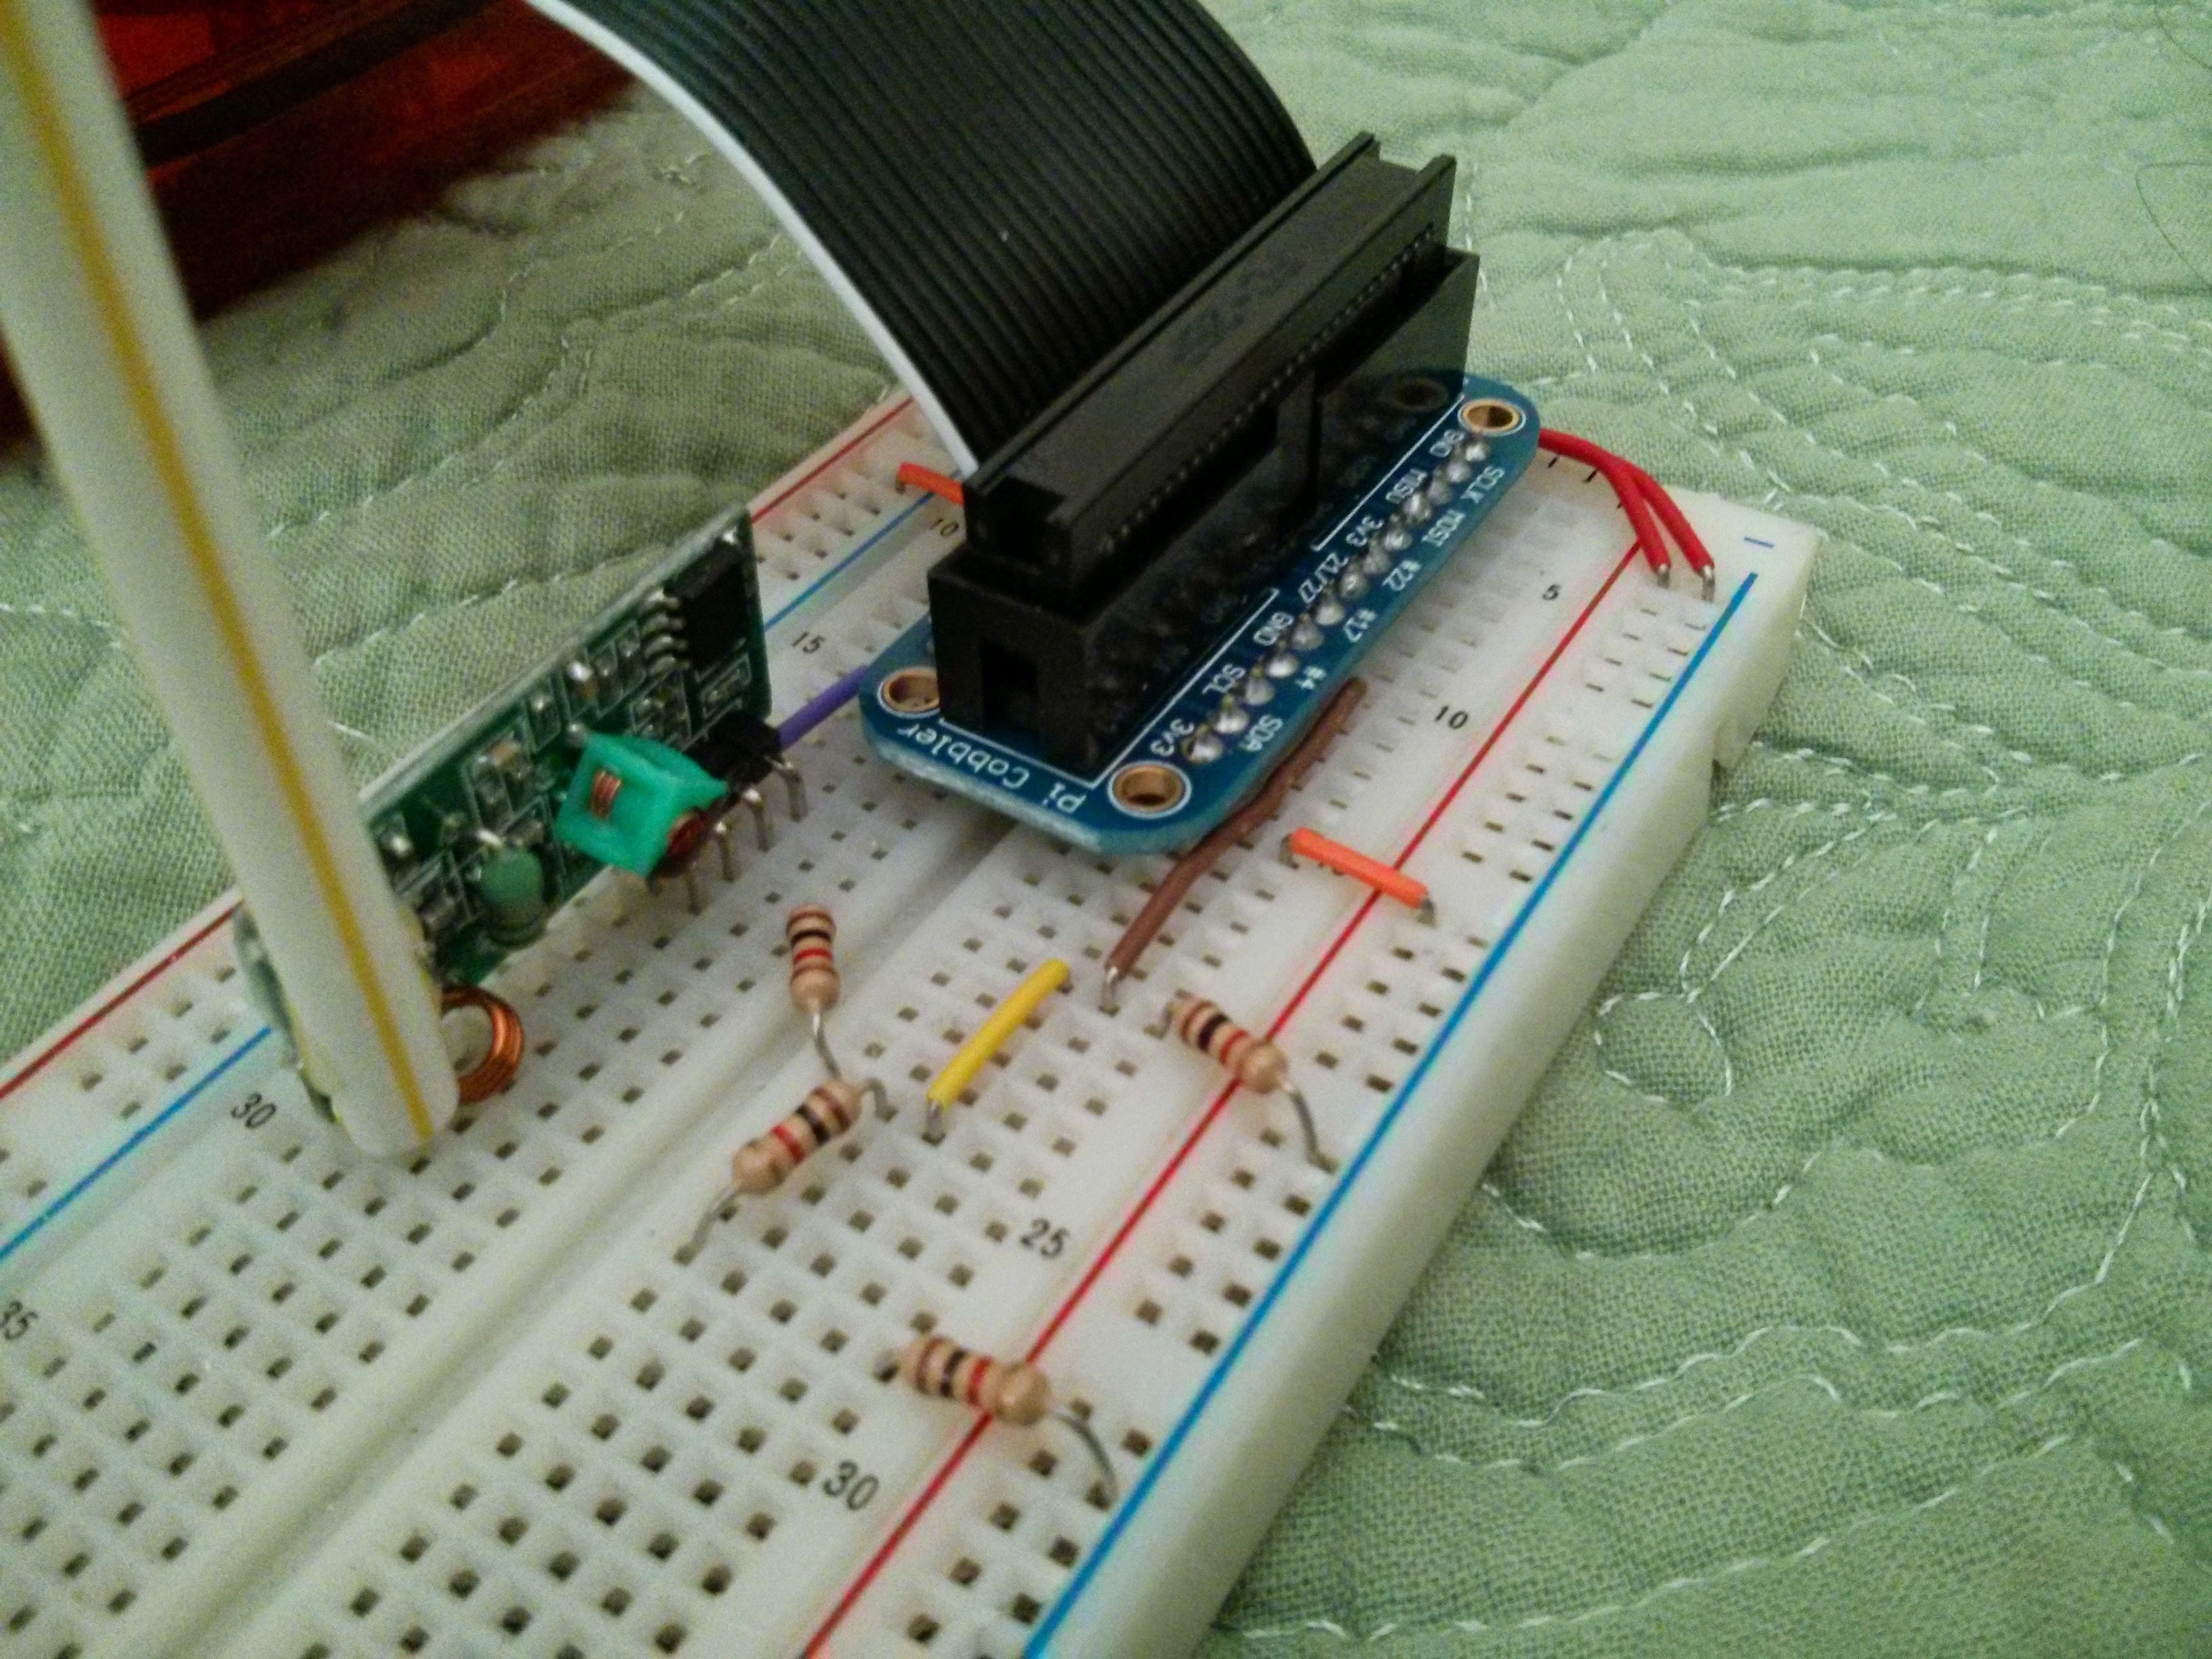
\includegraphics[width=\textwidth]{RaspberryPiRX.jpg}
		\caption{Raspberry Pi RX }
		\label{fig:pirx}
	\end{subfigure}%
	~ %add desired spacing between images, e. g. ~, \quad, \qquad etc.
	%(or a blank line to force the subfigure onto a new line)
	\begin{subfigure}[b]{0.3\textwidth}
		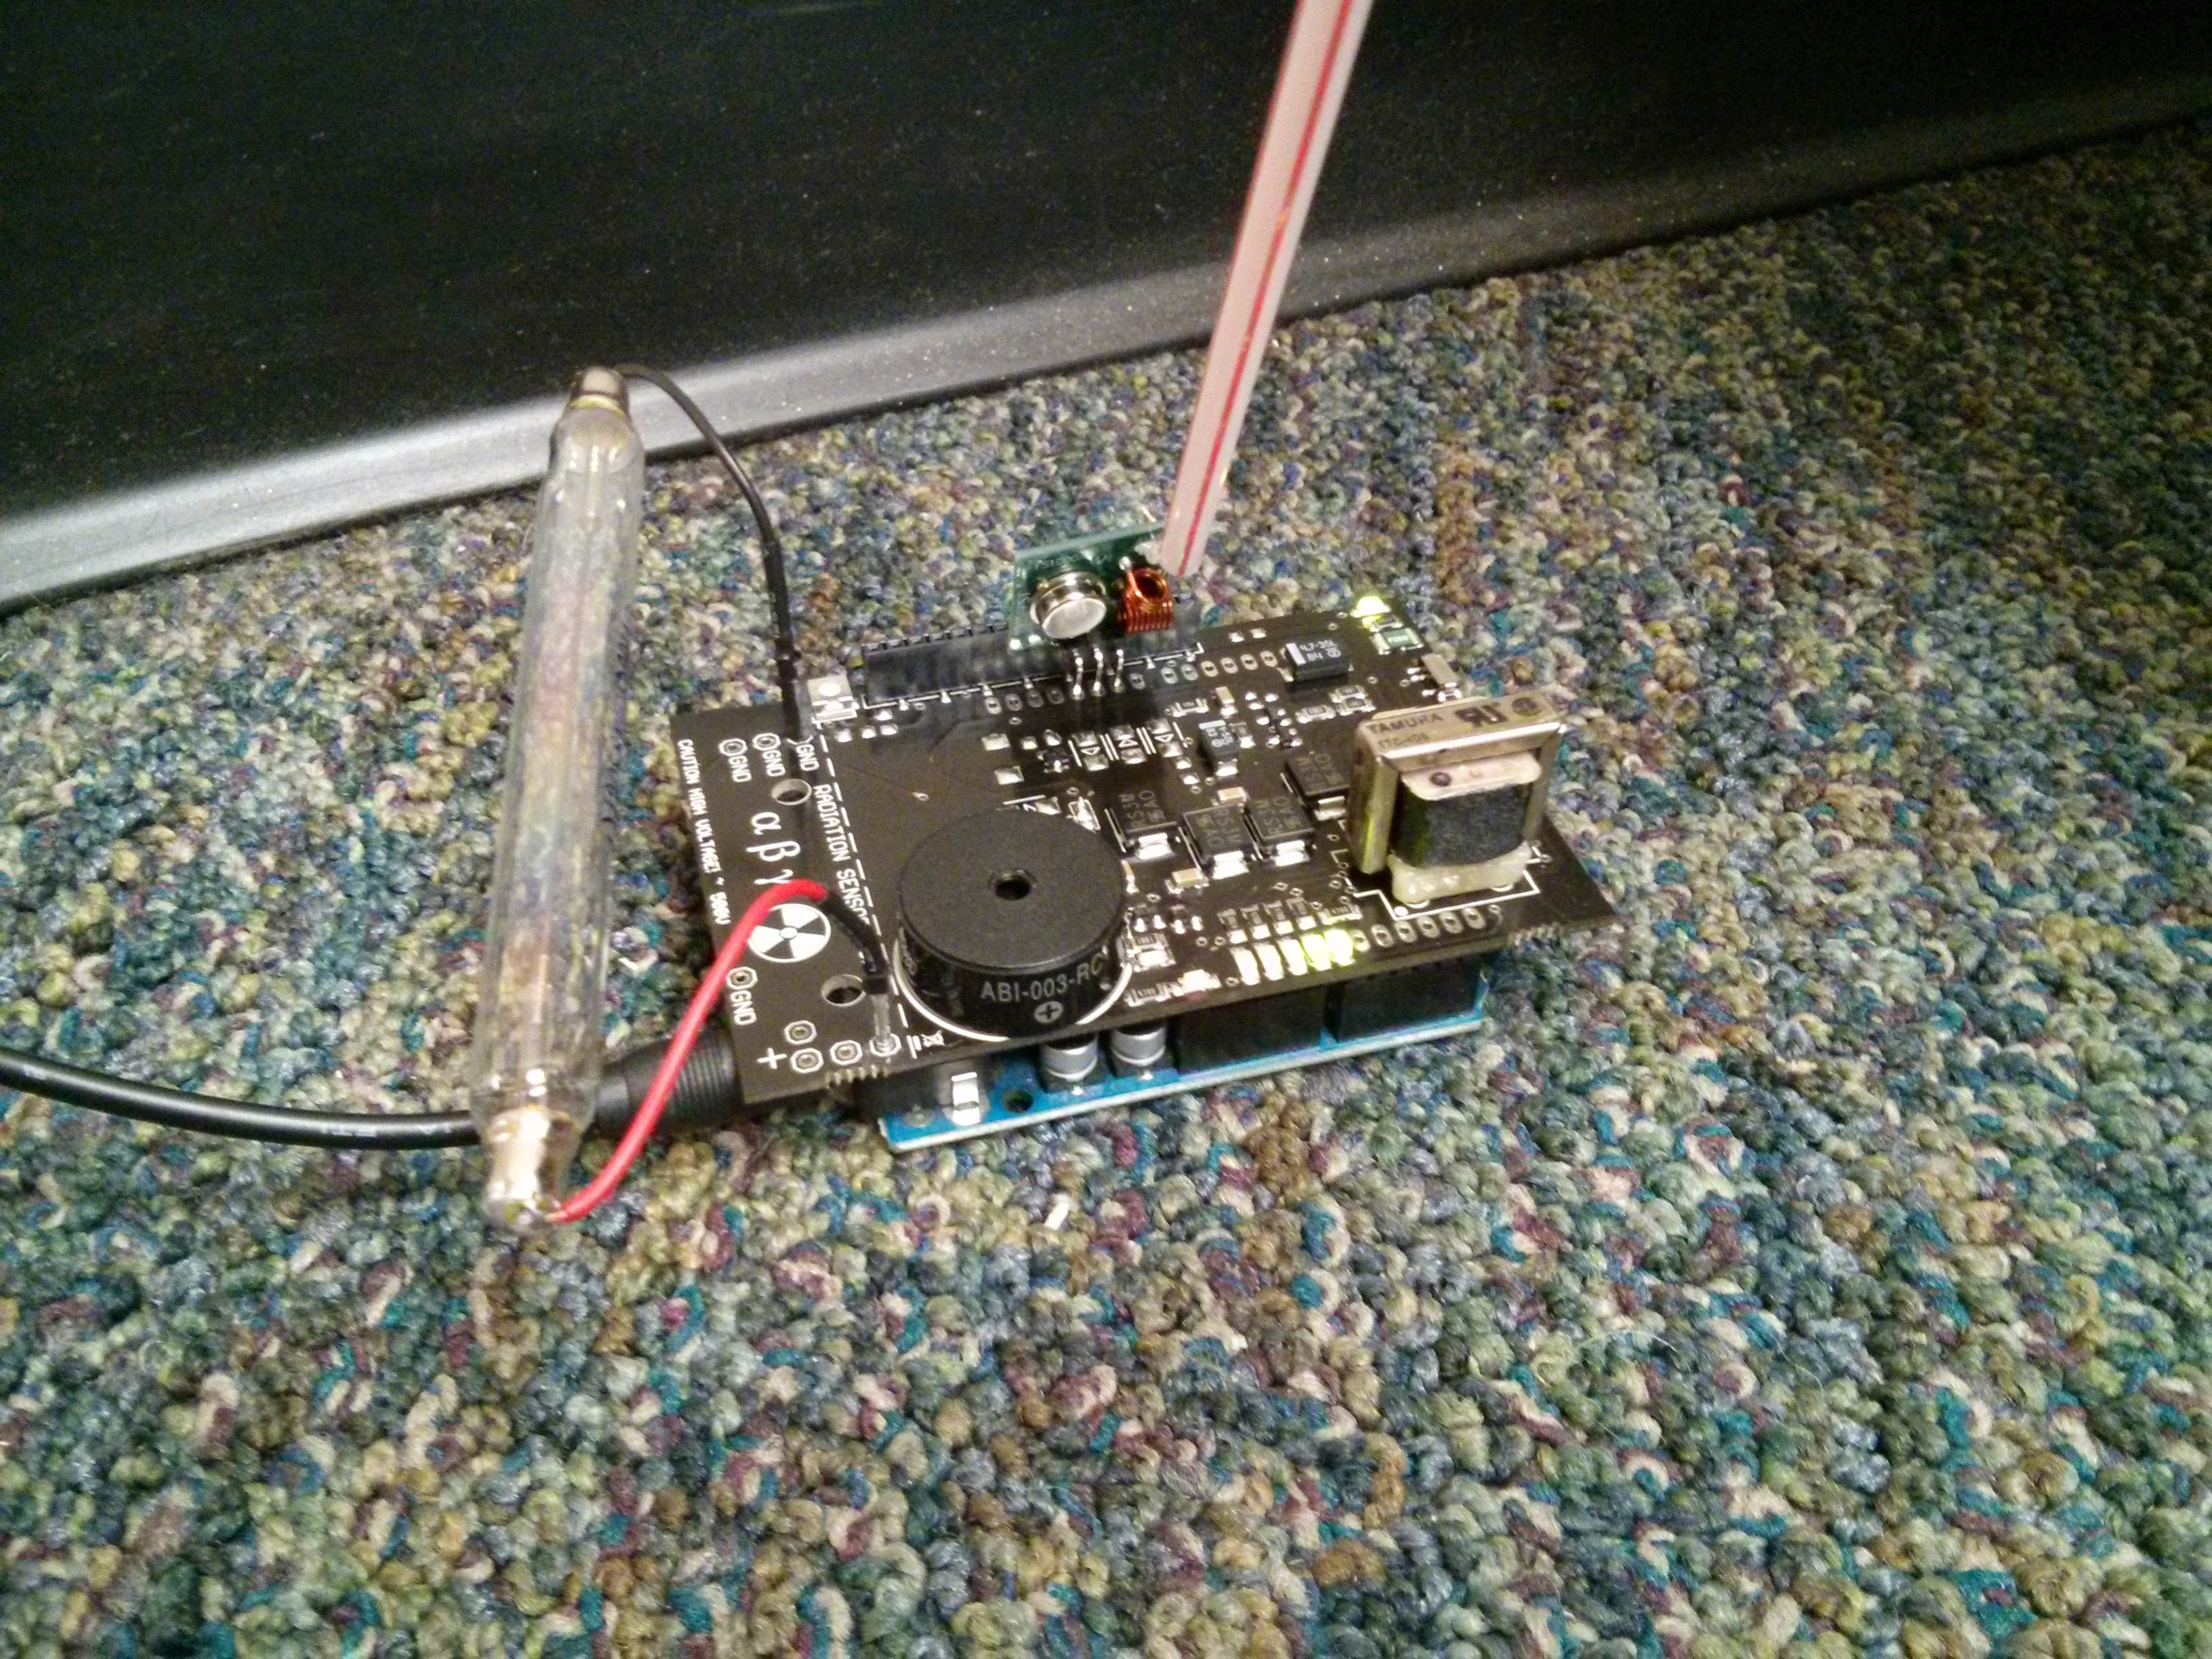
\includegraphics[width=\textwidth]{TransmitterArduinoCarpet.jpg}
		\caption{Arduino Transmitter}
		\label{fig:arduinotx}
	\end{subfigure}
	
	\caption{Prototype devices}\label{fig:txrx}
\end{figure}

\subparagraph{Power}
The device design has not reached the phase to focus on power consumption. The power regulators on the board consume the majority of power and therefore even an estimation of the final designs power consumption would not be possible. The unit is not able to run for elongated periods of time on batteries, although because the average current consumption is less than 100mA and is dependent on the amount of radiation it could be run from a solar panel.

\subparagraph{Cost}
Although the price per module was not reduced to the expected final product's cost, the device's cost per sensor is lower than commercially available sensors. The cost per module was reduced to about \$130 per transmitter mostly representing the cost of the Arduino Geiger Shield, with the Microcontroller unit and radio transmitter as the rest of the cost.

\subparagraph{Testing Range}
Range tests were conducted of the 433 MHz modules with a 173mm quarter wave whip antenna, with an indoor range of approximately 10m, it can be used in close range, but would fare much better outdoors. With a longer range due to less obstruction, approximately 30m is enough to mount receivers on lamp posts in urban areas, and attach the sensing transmitters to nearby buildings. Testing of multiple devices was also done, the receiver successfully took data from two sensors and differentiated counts based on their address. Through testing, of the 13588 rows transmitted, only 14 were not received properly.

\subparagraph{Server}

The server was built on two platforms based on usage scenarios. The Raspberry Pi (a small, inexpensive ARM based computer), and a Arduio. The Raspberry Pi also has the advantage of not needing anything but a 700mA power connector and an Ethernet port. This server is able to provide live data through a web page and internally through a SQL query-able database shown in Figure~\ref{webPage}. The Arduino based implementation (Figure~\ref{arduinorx}) is great for debugging and testing transmitter technologies before they need to be ported.

\begin{figure}[h]
	\centering
	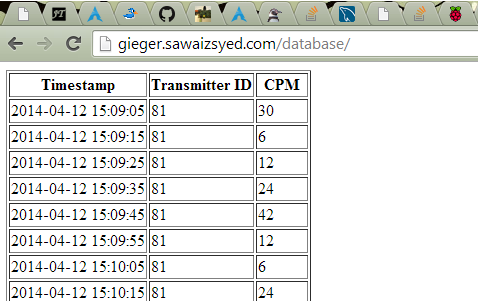
\includegraphics[width=0.5\textwidth]{WebDatabase.png}
	\caption{Web Page hosted on Raspberry Pi \label{webPage}}
\end{figure}

\begin{figure}[h]
	\centering
	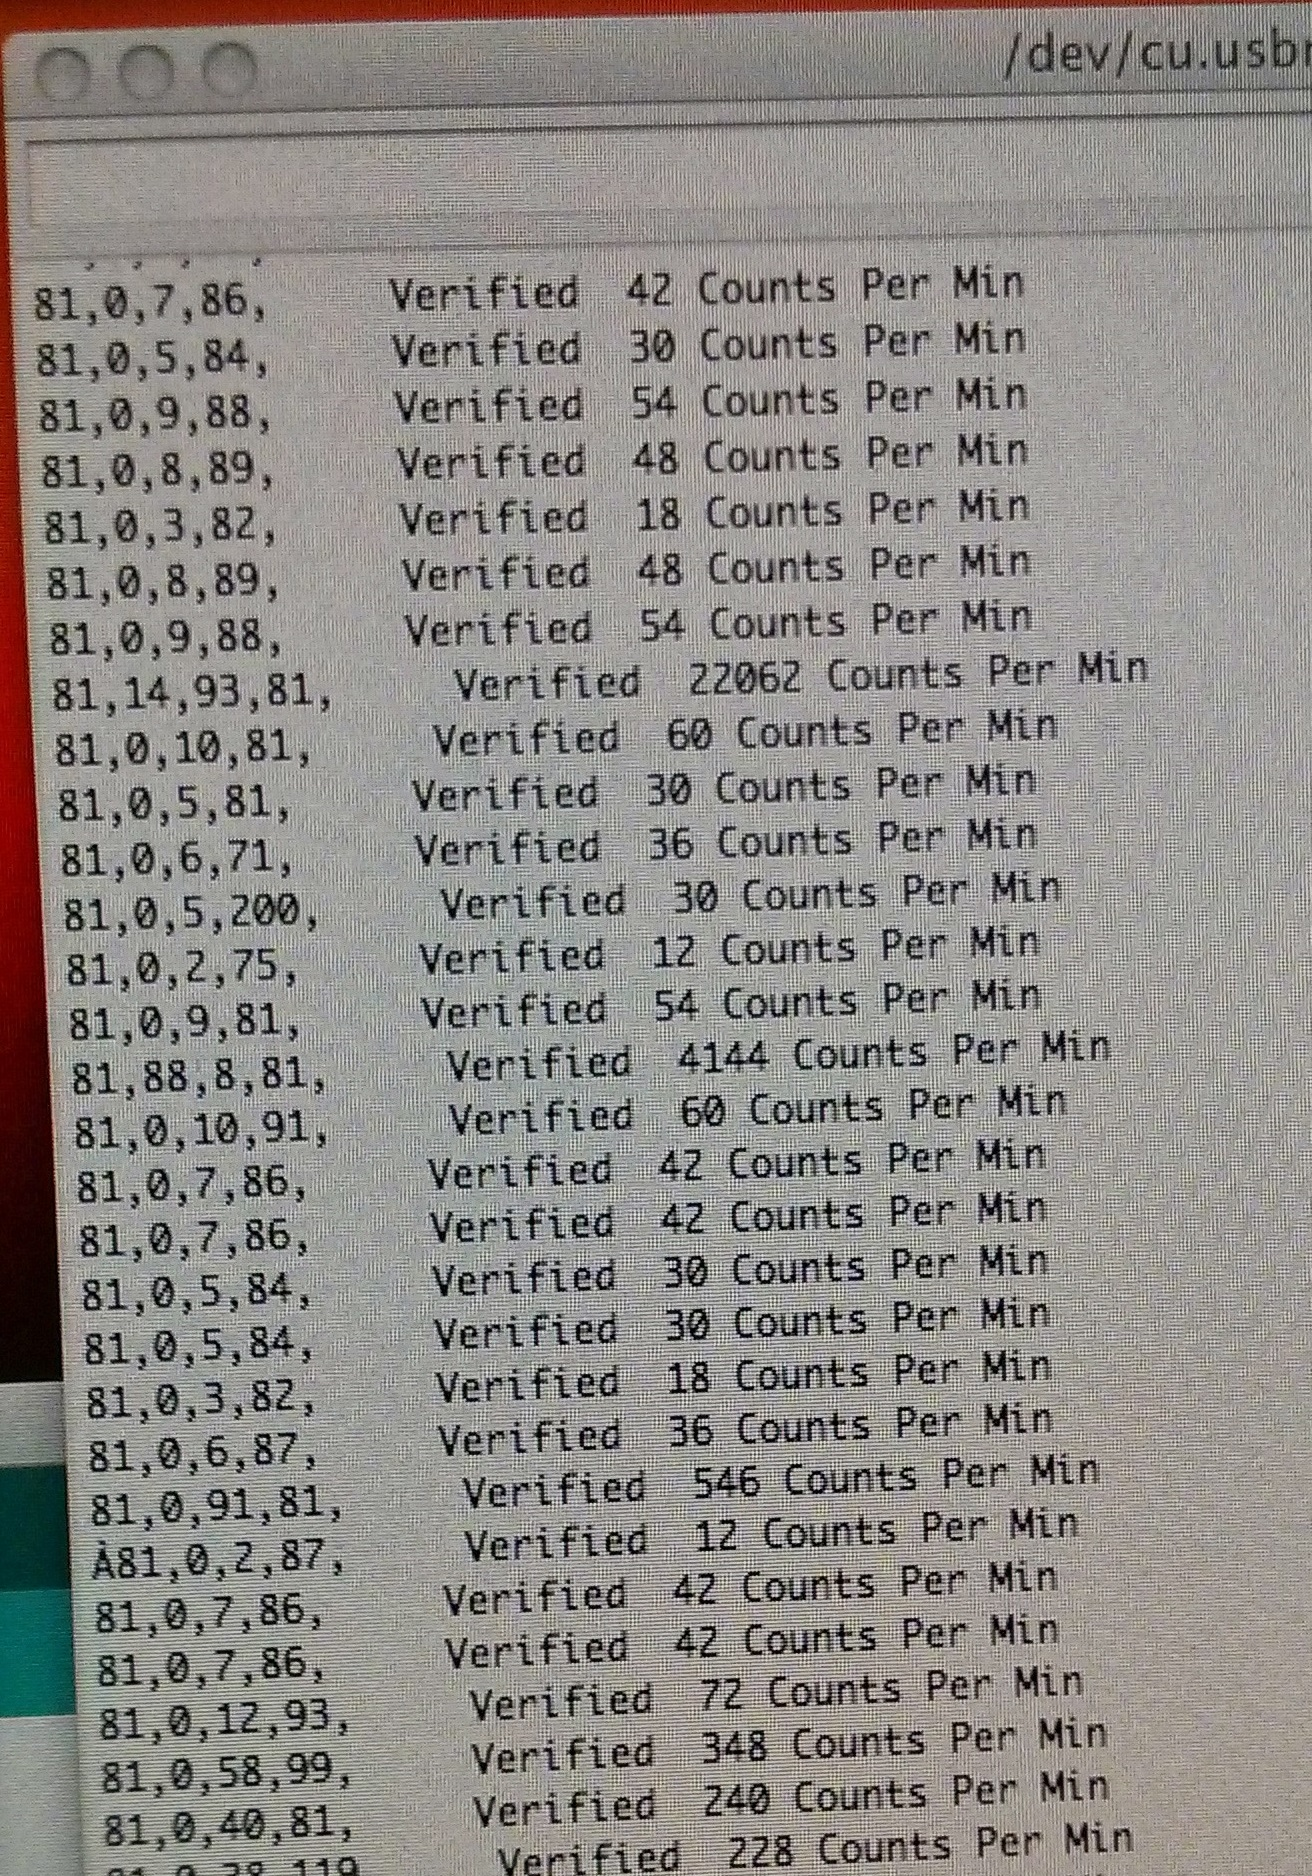
\includegraphics[width=0.5\textwidth]{ArduinoRX}
	\caption{Arduino Receiving Data \label{arduinorx}}
\end{figure}

\subparagraph{Documentation}
All the hardware and software specifications to this point are hosted on-line under open source licenses. There is also documentation of hardware setups and code hosted on an internal Wiki for parallel testing. This documentation allows upkeep of the code-base and devices by others.

\subsection*{Future Prospects}
The device still has a lot to be completed before it reaches the production quality needed. The prototype has shown significant promise and therefore steps to the final product should be few.

\subparagraph{Production}
Preparing the device for production, with custom made circuit boards, and reducing connectors, and part counts is the best way to reduce cost. For this to take place, components need to be ordered an assembled in prototypes of circuit boards and casing.

\subparagraph{Radio Transmitter}

For longer range modules using the NRF24L01+ chip based modules, are available and suggest a more concrete hardware link, and with their engineered antennas, provide longer range.

\section{Conclusion}

The design has taken many strides from the idea, as this is the initial prototype, the amount of progress is substantial. This lays a working model for future development. 

\pagebreak
\bibliographystyle{unsrt}
\bibliography{RadiationSensor}

\end{document}